\documentclass{standalone}

\usepackage{tikz}
\usetikzlibrary{positioning}


\begin{document}

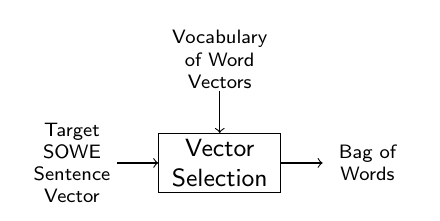
\begin{tikzpicture}[
	every node/.style={ text width=4em,
    					align=center,
                        font=\scriptsize\sffamily,
                        inner sep=1pt
                        },
	proc/.style= {draw,
    			  font=\small\sffamily,
                  inner sep = 2pt
    }
]
	\node (input) [inner sep=-4pt] {Target SOWE Sentence Vector};
    \node (selection) [proc, right = 1.5em of input]{Vector\\ Selection};
	\node (vocab) [above = 1.5em of selection]{Vocabulary of Word Vectors};
    \node (output) [inner sep=-4pt, right=1.5em of selection] {Bag of Words};
    \draw[->] (input) -- (selection);
    \draw[->] (vocab) -- (selection);
    \draw[->] (selection) -- (output);
\end{tikzpicture}

\end{document}